\titledquestion{Théorie des graphes}

Après une tempête de neige exceptionnelle, toutes les routes entre les villages de votre région sont enneigées.
Vous devez décider quelles routes déneiger pour que tous les villages soient reliés entre eux, tout en minimisant le coût total de déneigement.
Le réseau routier est représenté ci-dessous, où chaque nombre indique le coût de déneigement (en milliers d'euros) pour chaque route :

\begin{center}
    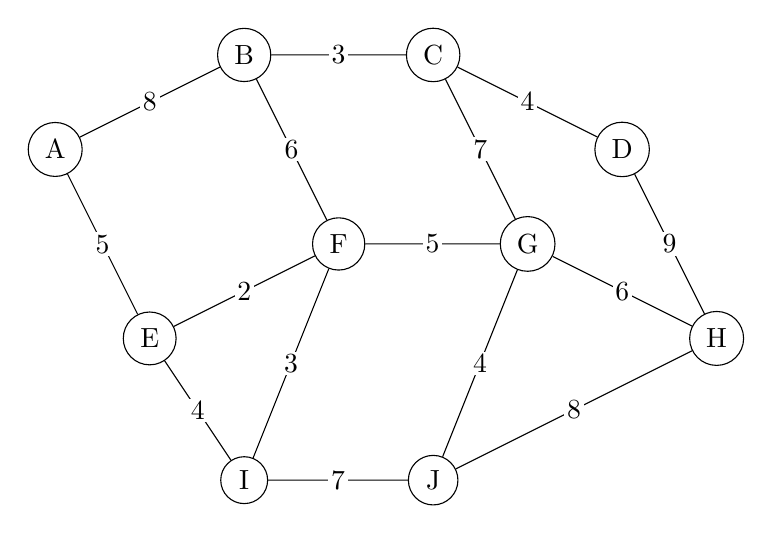
\begin{tikzpicture}[scale=1.2]
        \node[draw,circle] (A) at (0,2) {A};
        \node[draw,circle] (B) at (2,3) {B};
        \node[draw,circle] (C) at (4,3) {C};
        \node[draw,circle] (D) at (6,2) {D};
        \node[draw,circle] (E) at (1,0) {E};
        \node[draw,circle] (F) at (3,1) {F};
        \node[draw,circle] (G) at (5,1) {G};
        \node[draw,circle] (H) at (7,0) {H};
        \node[draw,circle] (I) at (2,-1.5) {I};
        \node[draw,circle] (J) at (4,-1.5) {J};

        \path [draw,-,>=stealth] (A) edge node[midway,fill=white,inner sep=1pt]{8} (B);
        \path [draw,-,>=stealth] (A) edge node[midway,fill=white,inner sep=1pt]{5} (E);
        \path [draw,-,>=stealth] (B) edge node[midway,fill=white,inner sep=1pt]{3} (C);
        \path [draw,-,>=stealth] (B) edge node[midway,fill=white,inner sep=1pt]{6} (F);
        \path [draw,-,>=stealth] (C) edge node[midway,fill=white,inner sep=1pt]{4} (D);
        \path [draw,-,>=stealth] (C) edge node[midway,fill=white,inner sep=1pt]{7} (G);
        \path [draw,-,>=stealth] (D) edge node[midway,fill=white,inner sep=1pt]{9} (H);
        \path [draw,-,>=stealth] (E) edge node[midway,fill=white,inner sep=1pt]{2} (F);
        \path [draw,-,>=stealth] (E) edge node[midway,fill=white,inner sep=1pt]{4} (I);
        \path [draw,-,>=stealth] (F) edge node[midway,fill=white,inner sep=1pt]{5} (G);
        \path [draw,-,>=stealth] (F) edge node[midway,fill=white,inner sep=1pt]{3} (I);
        \path [draw,-,>=stealth] (G) edge node[midway,fill=white,inner sep=1pt]{6} (H);
        \path [draw,-,>=stealth] (G) edge node[midway,fill=white,inner sep=1pt]{4} (J);
        \path [draw,-,>=stealth] (I) edge node[midway,fill=white,inner sep=1pt]{7} (J);
        \path [draw,-,>=stealth] (J) edge node[midway,fill=white,inner sep=1pt]{8} (H);
    \end{tikzpicture}
\end{center}

\begin{parts}
    \part Déterminez manuellement quelles routes déneiger pour que tous les villages soient reliés avec un coût minimal. Indiquez le coût total.
    \begin{solutionbox}{10.5cm}
        On cherche un arbre couvrant minimal (minimum spanning tree) qui relie tous les villages.
        
        On peut utiliser l'algorithme de Kruskal (ou Prim) mentalement :
        \begin{enumerate}
            \item Trier les arêtes par coût croissant : $EF(2)$, $BC(3)$, $FI(3)$, $CD(4)$, $EI(4)$, $GJ(4)$, $FG(5)$, $AE(5)$, $CG(7)$, $IJ(7)$, $AB(8)$, $DH(9)$
            \item Ajouter les arêtes une par une si elles ne créent pas de cycle :
            \begin{itemize}
                \item $EF$ (coût 2), $BC$ (coût 3), $FI$ (coût 3), $CD$ (coût 4) - ajouté
                \item $EI$ (coût 4) - crée un cycle avec $EF$ et $FI$, ignoré
                \item $GJ$ (coût 4), $FG$ (coût 5), $AE$ (coût 5) - ajouté
                \item $BF$ (coût 6), $GH$ (coût 6) - ajouté
            \end{itemize}
        \end{enumerate}
        
        L'arbre couvrant minimal contient les arêtes : $EF$, $BC$, $FI$, $CD$, $GJ$, $FG$, $AE$, $BF$, $GH$.
        
        Coût total : $2 + 3 + 3 + 4 + 4 + 5 + 5 + 6 + 6 = \boxed{38}$ milliers d'euros.
    \end{solutionbox}
    
    \part Considérons maintenant le problème avec un nombre $|V|$ de sommets et $|E|$ d'arêtes bien plus grand, de tel sorte que vous ne sachiez plus le résoudre à la main.
    Quel algorithme utiliseriez-vous pour trouver les routes à déneiger pour que tous les villages soient reliés avec un coût minimal ?
    Décrivez brièvement son principe et donnez sa complexité temporelle.
    \begin{solutionbox}{18cm}
        On utilise l'algorithme de Kruskal (ou l'algorithme de Prim) pour trouver un arbre couvrant minimal.
        
        \textbf{Algorithme de Kruskal :}
        \begin{enumerate}
            \item Trier toutes les arêtes par poids croissant.
            \item Initialiser une forêt (chaque sommet est son propre arbre).
            \item Pour chaque arête dans l'ordre croissant :
            \begin{itemize}
                \item Si les deux extrémités de l'arête sont dans des arbres différents, ajouter l'arête et fusionner les deux arbres.
                \item Sinon, ignorer l'arête (elle créerait un cycle).
            \end{itemize}
            \item S'arrêter quand on a $|V| - 1$ arêtes (un arbre a toujours $|V| - 1$ arêtes).
        \end{enumerate}
        
        \textbf{Complexité :} 
        \begin{itemize}
            \item Tri des arêtes : $\mathcal{O}(|E| \log |E|)$
            \item Pour chaque arête, vérifier si elle crée un cycle : $\mathcal{O}(\log |V|)$ avec une structure Union-Find efficace
            \item Total : $\mathcal{O}(|E| \log |E|) = \mathcal{O}(|E| \log |V|)$ (car $|E| \leq |V|^2$)
        \end{itemize}
        
        \textbf{Alternative : Algorithme de Prim}
        \begin{itemize}
            \item Commencer avec un sommet arbitraire.
            \item À chaque étape, ajouter l'arête de poids minimal qui connecte un sommet dans l'arbre à un sommet hors de l'arbre.
            \item Complexité : $\mathcal{O}(|E| + |V|\log|V|)$ avec une file de priorité efficace.
        \end{itemize}
    \end{solutionbox}
\end{parts}
